%; whizzy chapter
% -initex iniptex -latex platex -format platex -bibtex jbibtex -fmt fmt
% 以上 whizzytex を使用する場合の設定。


%     Tokyo Debian Meeting resources
%     Copyright (C) 2008 Junichi Uekawa

%     This program is free software; you can redistribute it and/or modify
%     it under the terms of the GNU General Public License as published by
%     the Free Software Foundation; either version 2 of the License, or
%     (at your option) any later version.

%     This program is distributed in the hope that it will be useful,
%     but WITHOUT ANY WARRANTY; without even the implied warranty of
%     MERCHANTABILITY or FITNESS FOR A PARTICULAR PURPOSE.  See the
%     GNU General Public License for more details.

%     You should have received a copy of the GNU General Public License
%     along with this program; if not, write to the Free Software
%     Foundation, Inc., 51 Franklin St, Fifth Floor, Boston, MA  02110-1301 USA

%  preview (shell-command (concat "evince " (replace-regexp-in-string "tex$" "pdf"(buffer-file-name)) "&"))
% 画像ファイルを処理するためにはebbを利用してboundingboxを作成。
%(shell-command "cd image200804; ebb *.png")

%%ここからヘッダ開始。

\documentclass[mingoth,a4paper]{jsarticle}
\usepackage{monthlyreport}

% 日付を定義する、毎月変わります。
\newcommand{\debmtgyear}{2008}
\newcommand{\debmtgmonth}{6}
\newcommand{\debmtgdate}{21}
\newcommand{\debmtgnumber}{41}

\begin{document}

\begin{titlepage}
\thispagestyle{empty}

% タイトルページ:編集必要な部分は最初のマクロに飛ばすこと

\vspace*{-2cm}
第\debmtgnumber{}回 東京エリア Debian 勉強会資料

\hspace*{-2.4cm}
\includegraphics[width=210mm]{image200801/2008title.eps}\\
\hfill{}\debmtgyear{}年\debmtgmonth{}月\debmtgdate{}日

\end{titlepage}

\dancersection{Introduction}{岩松 信洋}
 
 今月のDebian勉強会へようこそ。これからDebianの世界にあしを踏み入れると
 いう方も、すでにどっぷりとつかっているという方も、月に一回Debianについ
 て語りませんか?

 Debian勉強会の目的は下記です。

\begin{itemize}
 \item \underline{Debian Developer} (開発者)の育成。
 \item 日本語での「\underline{開発に関する情報}」を整理してまとめ、アップデートする。
 \item \underline{場}の提供。
 \begin{itemize}
  \item 普段ばらばらな場所にいる人々が face-to-face で出会える場を提供
	する。
  \item Debian のためになることを語る場を提供する。
  \item Debianについて語る場を提供する。
 \end{itemize}
\end{itemize}		

 Debianの勉強会ということで究極的には参加者全員がDebian Packageをがりがり
 と作るスーパーハッカーになった姿を妄想しています。情報の共有・活用を通し
 て Debianの今後の能動的な展開への土台として、「場」としての空間を提供す
 るのが目的です。

以上を目的とした、2008 年アジェンダです:
\begin{enumerate}
 \item 新年会「気合を入れる」
 \item Open Source Conference Tokyo (3/1)
 \item データだけのパッケージを作成してみる、
       ライセンスの考え方 (David Smith)
 \item バイナリ一つのパッケージを作成してみる (吉田@板橋)\\
       バージョン管理ツールを使いDebianパッケージを管理する(git)\\
       アップストリームの扱い(svn/git/cvs)(岩松 信洋さん)
 \item バイナリの分けたパッケージの作成。(前田さん)\\
       バイナリの分け方の考え方、アップグレードなどの運用とか。
 \item パッケージ作成(dpatch/debhelperで作成するパッケージ)(小林儀匡さん)\\
       man の書き方(roff or docbook)(でんさん)
 \item パッケージ作成(kernel patch、kernel module)
       、Debconf発表練習
 \item Debconf アルゼンチン、共有ライブラリパッケージ作成

 \item Open Source Conference Tokyo/Fall、
       デーモン系のパッケージの作成、latex、 emacs-lisp、フォントパッケージ
 \item パッケージの cross-compile の方法、amd64 上で i386 のパッケージと
       か、OSC-Fall報告会、Debconf報告会
 \item 国際化 po-debconf / po化 / DDTP
 \item 忘年会
\end{enumerate}


\newpage

\begin{minipage}[b]{0.2\hsize}
 \definecolor{titleback}{gray}{0.9}
 \colorbox{titleback}{\rotatebox{90}{\fontsize{80}{80} {\gt デビアン勉強会} }}
\end{minipage}
\begin{minipage}[b]{0.8\hsize}
\hrule
\vspace{2mm}
\hrule
\tableofcontents
\vspace{2mm}
\hrule
\end{minipage}


\dancersection{事前課題}{岩松 信洋}

今回の事前課題は以下です。

\begin{enumerate}
 \item 「debhelper に追加してほしい機能/あったらいい機能」
 \item 「 Debian を使っていて他の distro にあるこの機能/パッケージがあれば…と思ったこと」
\end{enumerate}

この課題に対して提出いただいた内容は以下です。

\subsection{吉田@板橋}

お題:Debian を使っていて他の distro にあるこの機能/パッケージがあれば…
と思ったこと

1.ドライバーディスク機能

redhat系ディストリービューションにあるドライバーディスク機能は欲しいです
ね。特にDISK関連のドライバは無いとお手上げなので。
たびたび武藤さんの手(スペシャルカーネル入りiso作成)を煩わせないためには、
あるといいかなと思います。
#どっちみちドライバディスク作成で手が煩わされるかな(笑)
インストール後は、あまり吊し(Debian純正)のカーネルを使わないので困らない
のですが。次善はlenny等を入れて強制ダウングレードするのが手かな。

2.Xの自動起動停止

runlevelで制御したいとまでは言いませんが...
基本はXなしで速く、マウスなしでログイン
必要ならXを上げるというサーバっぽい運用が行いにくいです。


\subsection{前田 耕平}

「Debian を使っていて他の distro にあるこの機能/パッケージがあれば…と
思ったこと」

Linuxじゃなくて、AIXなら楽だなぁと思う機能はあります。

\begin{itemize}
 \item LVM&ファイルシステムの拡張がAIXくらい楽にできれば良いなぁと思うことしばしば。
 \item システムバックアップの取得方法。mksysbコマンドのように楽に取れれば良いですね。
 \item エラーログの機能。errptコマンドでエラー情報を整形して表示できるのも良いです。
\end{itemize}

スキルレベルを標準化して運用要員を揃えるのなら、AIXは良いですね。自宅
では使いたくないですけど。w


\subsection{あけど}

「 Debian を使っていて他の distro にあるこの機能/パッケージがあれば…と
思ったこと」

ずばり、「Hinemos」です。http://www.hinemos.info/
Redhat で動いてるくらいだからDebianで動かすのは難しくなさそうですが、aptに慣れてしまうとdebパッケージであれば…と思ってしまいます。

\subsection{山本 浩之}

「Debian を使っていて他の distro にあるこの機能/パッケージがあれば…と
思ったこと」

TOMOYO Linux も公式に入ったことですし、AppArmor も早く公式に入って、セ
キュリティ・パッケージを強化すると嬉しい人が多そう。

\subsection{藤沢 理聡}


「Debian を使っていて他の distro にあるこの機能/パッケージがあれば…と思っ 
たこと」

これまでサーバにしか使ってこなかったので、機能面の不足はあんまり感じたこと 
ありません。
機能ではありませんが、不足を最も感じていたのは認識してもらえないハードが 
RedHat系より
多いんじゃないか、ということです。実際のところはどうかわかりません 
が、「RedHatでは
認識したんだけど……」と思うことは少なからずありました。とはいっても、2年以上 
前の
ことなので、既に改善されているのかもしれませんが。

\subsection{小林 儀匡}

「debhelper に追加してほしい機能/あったらいい機能」

Bug\#45614として提案されているdh\_{}alternativesが欲しいです。
alternativesを使用するパッケージを作成する場合、
ほとんどテンプレート化されているpostinstとprermと自分で書く必要がありますが、
メンテナスクリプトは極力メンテナに書かせないほうがよい気がするので……。


\subsection{日比野 啓}

「debhelper に追加してほしい機能/あったらいい機能」

perl module のパッケージを作ることが多いので、
perl のプログラムでも、バイナリにおける dh\_{}shlibdeps みたいに
ライブラリの依存関係の検知を支援してくれるような機能が欲しいです。

Debian を使っていて他の distro にあるこの機能/パッケージがあれば…と思ったこと

Debianというよりはlinuxの話かもしれませんが、
AIXのerrptのような厳密なチェック機能はすばらしいと思います。
あとは、FreeBSDのktraceがちょっとうらやましいと思ったことがあります。
だいぶ昔のなのでうろおぼえなんですが、kernelの中までtraceしてくれたような。

\subsection{岩松 信洋}

「Debian を使っていて他の distro にあるこの機能/パッケージがあれば…と思ったこと」

rpm にはドキュメントはインストールしないというオプションがあるのですが、Debian にはないので
インストール時に選択できるようにしてほしいです。
あと、他のディストリにはサポートしているのに Debian がサポート対象になっていないソフトウェアとか
けっこうあって(サイボウズさんとか)、それだけでDebianが使えないというのが悲しいです。

%%% trivia quiz
\dancersection{Debian Trivia Quiz}{岩松 信洋}

ところで、みなさん Debian 関連の話題においついていますか?Debian関連の話
題はメーリングリストをよんでいると追跡できます。ただよんでいるだけではは
りあいがないので、理解度のテストをします。特に一人だけでは意味がわからな
いところもあるかも知れません。みんなで一緒に読んでみましょう。

debian-devel-announceに流れた内容と Debian Project News からです。

\begin{multicols}{2}
 \subsection{debian-devel-announce}
 \url{debian-devel-announce@lists.debian.org}への投稿内容からです。

 \santaku
 {Debian.ch(スイス連邦のDebianユーザグループ)の体制が変わりました。どうなったでしょう。}
 {前会計が辞任したので、Martin F. Krafft が会計になりました。}
 {会計を全てスイス銀行の管理下に置かれます。}
 {スイス連邦のPascal Couchepin大統領がDebianユーザになりました。}
 {A}

 \santaku
 {2008年6月5日に新しい Debian Policy がリリースされました。バージョン番号はいくつでしょうか。}
 {3.1415}
 {3.8.0.0}
 {4.0.0.0}
 {B}
 
 \santaku
 {Debian installer lenny beta 2がリリースされたのはいつでしょうか。}
 {実は上川さんの誕生日、5月22日}
 {2008年6月1日}
 {2008年6月10日}
 {C}

 \subsection{Debian Project News - May 26th, 2008}
 \url{http://www.debian.org/News/weekly/2008/03/}への投稿内容からです

 \santaku
 {Perl の新しいバージョンの移行が完了しました。lennyに入る Perl のバージョンは? }
 {5.10}
 {5.20}
 {Perl-next-1.0}
 {A}

 \santaku
 {DPL から Bits from the DPL が出ました。あれ?今のDPLって?}
 {Sam Hocevar}
 {Martin Michlmayr}
 {Steve McIntyre}
 {C}

 \santaku
 {OpenSSHの DSA-1571 で影響を受けたパッケージ数はいくつでしょうか。}
 {20}
 {200}
 {2000}
 {A}

 \santaku
 {Debian Game team がデータの大きいサイズのパッケージについて提案したことは?}
 {データはP2Pで配信しようぜ!}
 {データはデータでアーカイブを分けようぜ!}
 {データは与えられるものではなく、与えるものだ!削除しましょう。}
 {B}

 \subsection{Debian Project News - June 9th, 2008}
 \url{http://www.debian.org/News/weekly/2008/04/}への投稿内容からです

 \santaku
 {ftp-master teamが編成されました。FTP MasterはJoerg Jaspertと誰になったでしょう?}
 {Ryan Murray}
 {Junichi Uekawa}
 {Kenshi Muto}
 {A}

 \santaku
 {debconf の翻訳が完了一番乗りした国は?}
 {フランス}
 {日本}
 {実は翻訳状況の表示不具合で、まだ一番乗りはいません}
 {A}

 \santaku
 {debconf の翻訳が遅れていて、CFH を出した国は?}
 {ドイツ}
 {日本}
 {実は翻訳状況の表示ミスで、遅れていませんでした}
 {A}

 \santaku
 {Bastian Venthur と Noel Koetheレポートを出したイベントは?}
 {BSDCan 2008}
 {LinuxWorld Expo/Tokyo 2008}
 {LinuxTag 2008}
 {C}

\end{multicols}

\dancersection{最近のDebian関連のミーティング報告}{岩松 信洋}
\subsection{東京エリアDebian勉強会40回目報告}

% (query-replace-regexp "<.*?>" "")
% (query-replace-regexp "^[	 ]\+" "")


東京エリアDebian勉強会報告。 5月の第40回東京エリアDebian勉強会を実施しました。  
今回の参加者は あけどさん、後藤さん、やまねさん、前田さん、沖中さん、 岩松さん、野村健太郎さん、堀内寛之さん、 小林儀匡さん、吉田@板橋さん、山本 浩之さん、 山本琢さん、福永さん、でん@相模原さん、奥野さん、 藤沢理聡さん、日比野 啓さん、荒木さん、 吉藤さん、上川の20人でした。

まず最初に最近のミーティングの報告を行いました。 台湾で行われたeeePC Open Source Developer's Conference の報告を簡単に行いました。

今回のクイズは小林さんが出題しました。 3問でだいたい全員不正解になるという勢いでした。
事前課題を紹介しました。 いろいろな話題が出ました。 ゴールデンウィークにさまざまなハックが行われていたようですね。

2008年のテーマはDEBパッケージの開発・管理に関連した内容ですが、 3回目のテーマとして前田さんが複数パッケージを生成するソースパッケージについて紹介しました。 debhelper の魔窟をすこし垣間見たようです。
OpenSSLの脆弱性の問題について議論しました。 いろいろな視点から検討し、問題の深刻さと、 どう公報するのがよいかについて議論しました。 また、SSHのキーの仕組みにはrevokeする方法が現在はなくて いちいち自分でいれかえる必要があるため大変だ、 ssh の鍵が脆弱ということで、 Debianで管理している範囲に影響が限定されないため、 パッチの配布だけでは解決しないところが困難だねという話題が出ました。

最近の kFreeBSD, nexenta, Hurd, SuperH について紹介して終了しました。

今回も宴会は駒忠にて開催しました。おばちゃんにまたきてね、と言われました。


\dancersection{パッケージ作成(debhelper、CDBS、dpatch、quiltを用いたパッケージ作成)}{小林儀匡}
\label{sec:dpatchdebhelper}
\index{cdbs} 
\index{debhelper} 
\index{quilt} 

\subsection{はじめに}

この文書では、
まずDebianパッケージのビルドの流れとdebian/rulesの各ターゲットの役割を概観した上で、
debhelperやCDBSを用いてdebian/rulesをメンテナンスしやすくする方法を説明します。
次に、開発元のソースコードに対する変更をメンテナンスしやすいかたちで加える方法として、
パッチ管理ツールであるdpatchとquiltの使い方を説明します。

一般的なDebianパッケージの作成方法に興味のある読者を対象としています。

\subsection{前回までのおさらい}

これまでにパッケージの作成について学んだことを整理してみましょう。
簡単にまとめてしまえば、以下のようになるのではないでしょうか。

\begin{itemize}
 \item debパッケージの作成には、ソースツリーにdebian/changelog、debian/control、debian/copyright、debian/rulesという4つのファイルが最低限必要。
\begin{description}
 \item[debian/changelog] ソースファイルの変更履歴。
    最初のエントリが現在のバージョンに関する記述となり、
    ビルドされるパッケージのバージョン情報もここから抽出される。
 \item[debian/copyright] 著作権・ライセンス情報を収めたファイル。
    バイナリパッケージの\texttt{/usr/share/doc/$<$バイナリパッケージ名$>$/copyright}にインストールされる。
    現在のところ、debianディレクトリにありながら機械的に処理されることのない珍しいファイルで、
    書式も厳格には決められていない\footnote{書式を定めて機械可読にする議論がなされている。
    機械可読になった場合は、パッケージマネージャでライセンス情報を扱えるようになると考えられる。
    詳しくは\url{http://wiki.debian.org/Proposals/CopyrightFormat}を参照のこと。}。
 \item[debian/rules] ビルド方法を記述したGNU Make makefile。
 \item[debian/control] パッケージ (ソースパッケージおよびバイナリパッケージ) のメタ情報を指定するファイル。
    バージョン番号や作成日時など、バージョンごとに異なる情報はdebian/changelogに書かれるため、
    debian/controlには変更頻度の比較的低いメタ情報のみが収められる。
    また、生成されるソースパッケージとすべてのバイナリパッケージの名前もここで指定される。
    ファイルは空行で複数の段落に区切られており、
    そのうち最初の段落がソースパッケージおよびすべてのバイナリパッケージ用、
    その後に続く1つ以上の段落が各バイナリパッケージ用である。
\end{description} 
 \item \texttt{dh\_make}を使うと、これらのファイルや、
  ビルドに用いられるその他の設定ファイルの雛形を作成してくれる。
  それらを適当に編集してdebuildを実行するとソースパッケージおよびバイナリパッケージを作成できる。
\end{itemize}

一通りのパッケージ作成の流れや、
debian/rules以外のファイルの内容は何となく分かったかと思います。
しかし、debhelperのコマンドが連ねられているdebian/rulesについては、
実際のところどのようなことをしており、
どのような流れでパッケージが作られているのかは、おそらくまだ理解できていないと思います。
また、パッケージをさらに細かく設定し、より洗練されたものにする方法も分からないでしょう。

そこで、今回は、debian/rulesとdebhelperの各コマンドの内容を説明し、
パッケージがどのような過程を経てビルドされているのかを明らかにします。
その上で、debhelperやCDBSを用いて、
Debian Policy Manual (\emph{debian-policy})に準拠したパッケージをメンテナンスしやすいかたちで作成する方法を説明します。
また、開発元のソースコードに対する変更をメンテナンスしやすいかたちで加える方法として、
パッチ管理ツールであるdpatchとquiltの使い方を説明します。

まずビルドの流れについて見ていくことから始めましょう。

% ソースパッケージの構成とソースツリーについても語るべき?

% debian-policyに準拠したDebianパッケージとしてはもちろん必要だが、
% debian/changelogは現段階ではパッケージのビルド自体には不要?

\subsection{debパッケージのビルド手順}

debuildなどのパッケージビルドツールでは、大まかに言うと、
一般的に次のような手順でパッケージをビルドします。

\begin{enumerate}
 \item ビルド環境を整備する。
 \item 不要なファイルを削除する (\texttt{debian/rules clean})。
 \item ソースパッケージをまとめる (\texttt{dpkg-source -b $<$ディレクトリ名$>$})。
 \item バイナリパッケージにインストールするファイルをビルドする (\texttt{debian/rules build})。
 \item ビルドしたファイルをバイナリパッケージにまとめる (\texttt{debian/rules binary})。
 \item .changesファイルを作成する (\texttt{dpkg-genchanges})。
 \item パッケージに署名する。
\end{enumerate}

以下でこれらを詳しく説明します。

\subsubsection{ビルド環境を整備する}

実際にビルドを始める前に、まずはビルドのための環境を整える必要があります。

「ビルドのための環境を整える」と一口に言っても色々とありますが、
例えばソースパッケージの展開などが挙げられます。
ソースパッケージをビルドする場合は、
ソースパッケージを展開してソースツリーの状態にするところから始めなければなりません。
もちろんソースツリーでビルドする場合はこれは不要です。

また、
パッケージのビルドには、通常、様々なもの (コンパイラやライブラリなど) が必要となるので、
ビルド中にエラーにならないよう、それらの存在を確認しておく必要もあります。
必要となるパッケージは、ソースパッケージの場合は.dscファイルのBuild-Dependsフィールド、
ソースツリーの場合はdebian/controlのBuild-Dependsフィールドに書かれています。
ビルドツールによっては、ビルドに必要なパッケージを確認するだけでなく、
インストールされていない場合にインストールしてくれるものもあります。

また、pdebuildなどのようにchroot環境内でパッケージをビルドするツールは、
こういった作業の前にまずchroot環境を作ってそこに入るところから始めるでしょう。

\subsubsection{不要なファイルを削除する (\texttt{debian/rules clean})}

必要なパッケージが揃っていることを確認したところで、
不要なファイルを削除します。
一般に、以前のビルドで生成されたファイルがある場合はそれを削除して、
常に同じ状態からビルドできるようにすべきです。
debian/rulesのcleanターゲットをそのような目的で使うよう、
debian-policyにおいて定められています。

\subsubsection{ソースパッケージをまとめる (\texttt{dpkg-source -b $<$ディレクトリ名$>$})}

ソースパッケージを作成するタイミングとしては、不要なファイルを削除した後、
バイナリパッケージに含めるファイルのビルドに入る前が最もよいでしょう。
\texttt{dpkg-source}コマンドの\texttt{-b}オプションを使うと、
ソースツリーからソースパッケージを作成できます。

\subsubsection{バイナリパッケージにインストールするファイルをビルドする (\texttt{debian/rules build})}

ソースパッケージを作成し終えたらいよいよバイナリパッケージの作成に移ります。
バイナリパッケージの作成は大きく2段階に分けることができます。
最初の段階は、設定やコンパイルです。

Cなどの言語で書かれたプログラムやライブラリがパッケージに含まれている場合、
それらをインストール前にコンパイルして、
バイナリのプログラムやライブラリを作成する必要があります。
プログラムのビルドにGNU Autoconfを使用するようになっている場合は、
コンパイルの前にconfigureスクリプトを走らせて設定を行う必要もあるでしょう。

この手続きは、
バイナリのプログラムやライブラリを含んでいないパッケージについても必要になることが多いでしょう。
例えば、\LaTeX{}やSGMLなどの形式で書かれたドキュメントは、
HTMLやPostScript、PDFなどの配布に適した形式に変換してバイナリパッケージに含めるべきです。
また、ソースとなるデータを変換してインストール用のデータを作成する必要がある場合も、
通常はここでその変換を行います。

debian-policyでは、
このような、プログラムやライブラリの設定・コンパイルやデータの変換のために、
debian/rulesのbuildターゲットを使うよう指定されています。

% tarballからソフトウェアのインストールをしたことがあるかたは、
% 「./configure; make」のプロセスと言えばお分かりかと思います。

\subsubsection{ビルドしたファイルをバイナリパッケージにまとめる (\texttt{debian/rules binary})}

必要なファイルをすべてビルドしたところで、
それらを適切なパーミッションで適切な場所に配置し、
バイナリパッケージにまとめ上げる必要があります。
あっさりと書いてしまいましたが、
debian-policyに準拠するパッケージを手で作成しようとする場合には、
かなり複雑で面倒な作業を要求されるプロセスです。

このプロセスは、通常、
まずdebian/tmpを/と見なしてソフトウェア全体のインストール (「仮インストール」) を行い、
その上でdebian/tmp内の各ファイルを適切にdebian/$<$バイナリパッケージ名$>$に振り分け、
最後にdebian/$<$バイナリパッケージ名$>$をそれぞれバイナリパッケージ化する、
という流れで行います。
debian/$<$バイナリパッケージ名$>$をバイナリパッケージ化する際には、
パーミッションの調節やファイルの圧縮など、
しなければならないこと、推奨されていることが多数あります。
それらは後で詳述しますので、ここでは詳しい説明は省きます。

debian-policyでは、バイナリパッケージをまとめ上げるために、
debian/rulesのbinaryターゲットを使うよう指定されています。

\subsubsection{.changesファイルを作成する (\texttt{dpkg-genchanges})}

ソースパッケージとバイナリパッケージのファイルが一通り揃ったところで、
これらのファイルに関する情報をまとめた.changesファイルを作成する必要があります。
これには\texttt{dpkg-genchanges}コマンドが使用されます。

\subsubsection{パッケージに署名する}

私家版パッケージやテストビルドでは必要ありませんが、公式パッケージにする場合は、
最後にパッケージに署名する必要があります。
公式パッケージにしない場合でも、広く配布する場合には署名することをお勧めします。

署名は、.dscファイルと.changesファイルに対して行います。
.dscファイルにはソースパッケージの.tar.gzファイルと.diff.gzファイルのハッシュとサイズが書かれているので、
署名を施すことでこれらのファイルの品質を保証できます。
また、.changesファイルにはソースパッケージとバイナリパッケージのすべてのファイルのハッシュとサイズが書かれているので、
署名を施すことでこれらのファイルすべての品質を保証できます\footnote{厳密に言えば、
以前のバージョンと同一の.tar.gzファイルを使用している場合は、
.tar.gzファイルの情報は.changesファイルには記載されません。
したがって、この場合は.dscファイルを経由した間接的な保証となります。}。

署名には、通常、devscriptsパッケージに含まれているdebsignコマンドを使います。
このコマンドは、最初に.dscファイルに対する署名を行い、その後で、
.changes内の.dscファイルのエントリのハッシュやサイズを署名後の値に置換した上で、
.changesファイルに署名してくれます。

\subsection{debian/rulesのターゲット}

ビルド手順の説明から分かるかと思いますが、
debian/rulesには、パッケージのビルド時に必要となるターゲットがあります。
説明に登場したclean、build、binaryの他に、binary-archとbinary-indepも必須のターゲットです。
以下でこれらのターゲットの役割を簡単に示します (詳細はdebian-policyを参照してください)。

\begin{description}
 \item[clean]
    buildターゲットやbinaryターゲットで行った変更をすべて元に戻すためのターゲットです。
    ただし、生成されたバイナリパッケージの削除はすべきでありません。
    このターゲットはroot権限で呼び出す必要があるかもしれません。
 \item[build]
    バイナリパッケージに含めるプログラムやライブラリの設定・コンパイルやデータの変換に使用されるターゲットです。
    設定が対話的だとパッケージの自動ビルドができなくなるため、
    設定は非対話的なものでなければなりません。
    インストールパスなどの設定を対話的に行うようになっているソフトウェアについては、
    設定用のプログラムの書き換えなどで対応してください。
    このターゲットでは、root権限が必要な操作を行ってはなりません。
 \item[binary]
    binaryターゲットは、
    buildターゲットでビルドされたバイナリパッケージをまとめ上げるのに使用されます。
    binaryターゲットは、通常、
    binary-archターゲットとbinary-indepターゲットに依存するだけとなります。
    このターゲットはroot権限で呼び出されなくてはなりません。
 \item[binary-arch]
    ビルドされたファイルから特定アーキテクチャ用バイナリパッケージを生成するためのターゲットです。
    パッケージに含めるファイルをビルドするターゲットとして、
    buildターゲット (または定義されている場合はbuild-archターゲット) に依存するようにしておくべきです。
    このターゲットはroot権限で呼び出されなくてはなりません。
 \item[binary-indep]
    ビルドされたファイルからアーキテクチャ非依存バイナリパッケージを生成するためのターゲットです。
    パッケージに含めるファイルをビルドするターゲットとして、
    buildターゲット (または定義されている場合はbuild-indepターゲット) に依存するようにしておくべきです。
    このターゲットはroot権限で呼び出されなくてはなりません。
\end{description}

clean、build、binaryについては、
パッケージのトップレベルディレクトリ (debianディレクトリの親ディレクトリ) をカレントディレクトリとして実行するよう定められています。

\subsection{debhelperを使わないdebian/rules}

debian/rulesの必須ターゲットに関する規約を簡単に眺めたところで、
実際のパッケージのdebian/rulesの例を見てみましょう。
以下では、Debianパッケージ作成用のツールを何も使わずに実装した、
helloパッケージのdebian/rulesから抽出したコード (を一部改変したもの) を例に示します。

まずはcleanターゲットです。

\begin{commandline}
clean:
	rm -f build
	-$(MAKE) -i distclean
	rm -rf *~ debian/tmp debian/*~ debian/files* debian/substvars
\end{commandline}

簡単に読めますね。
以下のことをやっているだけです。

\begin{itemize}
 \item タイムスタンプとして使用したbuildファイルを削除する。
 \item ソフトウェアのMakefileのdistcleanターゲットを実行し、
  ソフトウェアのビルドで生成されたファイルを削除する。
 \item パッケージのビルド時にdebianディレクトリ内に作成されたファイルを削除する。
\end{itemize}

続いてbuildターゲットです。

\begin{commandline}
CC = gcc
CFLAGS = -g -Wall

ifeq (,$(findstring noopt,$(DEB_BUILD_OPTIONS)))
  CFLAGS += -O2
endif

build:
	./configure --prefix=/usr
	$(MAKE) CC="$(CC)" CFLAGS="$(CFLAGS)"
	touch build
\end{commandline}

GNU Makeのmakefileに慣れていないと、変数の設定の部分が分かりにくいかもしれませんが、
buildターゲット自体は非常に単純ですね。
ソフトウェアをソースからインストールしたことのあるかたならお馴染みの、
Autoconfを用いた一般的なCプログラムのビルド方法です。

最後に、binary、binary-arch、binary-indepの3つのターゲットです。

\begin{commandline}
package = hello
docdir = debian/tmp/usr/share/doc/$(package)

INSTALL_PROGRAM = install

ifeq (,$(findstring nostrip,$(DEB_BUILD_OPTIONS)))
  INSTALL_PROGRAM += -s
endif

binary-indep: build

binary-arch: build
	rm -rf debian/tmp
	install -d debian/tmp/DEBIAN $(docdir)
	$(MAKE) INSTALL_PROGRAM="$(INSTALL_PROGRAM)" \
		prefix=$(CURDIR)/debian/tmp/usr install
	cp -a NEWS debian/copyright $(docdir)
	cp -a debian/changelog $(docdir)/changelog.Debian
	cp -a ChangeLog $(docdir)/changelog
	cd $(docdir) && gzip -9 changelog changelog.Debian
	gzip -r9 debian/tmp/usr/share/man
	dpkg-shlibdeps debian/tmp/usr/bin/hello
	dpkg-gencontrol
	chown -R root:root debian/tmp
	chmod -R u+w,go=rX debian/tmp
	dpkg-deb --build debian/tmp ..

binary: binary-indep binary-arch
\end{commandline}

一つずつ手順を追っていけば、
以下のような手順でバイナリパッケージを生成していることが分かります。

\begin{enumerate}
 \item インストール先のディレクトリを準備する。
 \item ソフトウェアのMakefileのinstallターゲットで、
    インストール先のディレクトリにファイルをインストールする。
    環境変数\texttt{DEB\_BUILD\_OPTIONS}にnostripという文字が含まれていない場合は、
    インストール時に、オブジェクトファイルからシンボルを切り捨てる (stripする)。
 \item インストール先のドキュメント用ディレクトリに、
    ソフトウェアのドキュメントやdebian/copyrightをインストールする。
 \item インストール先のドキュメント用ディレクトリに、
    debian/changelogおよびソフトウェアのChangeLogを、
    それぞれchangelog.Debianおよびchangelogとしてインストールする。
 \item インストールしたchangelog.Debianおよびchangelogやマニュアルページを圧縮する。
 \item インストールしたバイナリファイルの、ビルドに使われたライブラリへの依存関係を調べて、
    debian/substvarsに変数\$\{shlibs:Depends\}を設定する。
 \item debian/controlを元にdebian/tmp/DEBIAN/controlを作成する。
    その際に、debian/control内の「\$\{shlibs:Depends\}」を、
    先に設定した変数の値で置換する。
 \item インストール先のディレクトリやファイルのパーミッションを適切に設定する。
 \item debパッケージにする。
\end{enumerate}

バイナリプログラム1つと付随データをバイナリパッケージ1つにインストールするだけなのに、
かなり複雑な手順を踏んでいます。
これは以下のような理由からです。

\begin{itemize}
 \item 以下のようなものに関してdebian-policyの規約に従う必要がある。
\begin{itemize}
 \item インストールすべきドキュメント
 \item インストールされたファイルのパーミッション
 \item 圧縮すべきファイル
 \item オブジェクトファイル内のシンボルの扱い
\end{itemize} 
 \item 依存関係の記述を簡単にするための変数「\$\{shlibs:Depends\}」を処理する必要がある。
 \item debian/tmp/DEBIAN以下に、debian/controlなどのパッケージのメタ情報を含むファイルや、
  メンテナスクリプトを入れなければならない。
\end{itemize}

バイナリパッケージ1つを生成するパッケージでさえこれだけの手順を踏まなければならないので、
様々なファイルを複数のバイナリパッケージに分けてインストールするようなパッケージの作成に、
かなり手間がかかるのは容易に想像できます。

\begin{screen}
\paragraph*{debファイルの内容}

dpkg-deb --buildがどのようにして複数のファイルを1つの「パッケージ」にまとめているか、
興味があるかもしれません。
そのような場合は、以下の実行例が参考になるでしょう。

\begin{commandline}
noritada[3:50]%  ls                       
hello_2.2-2_i386.deb
noritada[3:50]%  ar x hello_2.2-2_i386.deb
noritada[3:50]%  ls 
control.tar.gz	data.tar.gz  debian-binary  hello_2.2-2_i386.deb
noritada[3:50]%  cat debian-binary 
2.0
noritada[3:50]%  tar ztf control.tar.gz 
./
./control
noritada[3:50]%  tar ztf data.tar.gz 
./
./usr/
./usr/share/
./usr/share/doc/
./usr/share/doc/hello/
[snip]
./usr/share/man/
./usr/share/man/man1/
./usr/share/man/man1/hello.1.gz
./usr/bin/
./usr/bin/hello
\end{commandline}
\end{screen}

\subsection{debhelperを用いたdebian/rules}

debian-policyの規約に従ったDebianパッケージを容易に作成できるようにしてくれるのが、
debhelperです。
例として、先程のhelloパッケージに対してdebhelperを使用したhello-debhelperパッケージのdebian/rulesを見てみましょう。

まずはcleanターゲットです。

\begin{commandline}
clean:
	dh_clean
	rm -f build
	-$(MAKE) -i distclean
\end{commandline}

helloパッケージの場合とほぼ同じですが、
debianディレクトリの掃除に関しては\texttt{dh\_clean}というコマンドを使用していることが分かります。

次はbuildターゲットですが、これはhelloパッケージのものとまったく同じなので省略します。

最後に、helloパッケージではかなり複雑だった、
binary、binary-arch、binary-indepの3つのターゲットです。

\begin{commandline}
package = hello-debhelper

install: build
	dh_clean
	dh_installdirs
	$(MAKE) prefix=$(CURDIR)/debian/$(package)/usr install

binary-indep: install

binary-arch: install
	dh_installdocs -a NEWS
	dh_installchangelogs -a ChangeLog
	dh_strip -a
	dh_compress -a
	dh_fixperms -a
	dh_installdeb -a
	dh_shlibdeps -a
	dh_gencontrol -a
	dh_md5sums -a
	dh_builddeb -a

binary: binary-indep binary-arch
\end{commandline}

「dh\_」で始まるコマンド群で占められているのが分かります。
これらがdebhelperのコマンドです。
オプションやファイル名の指定などは部分的にはあるものの、
基本的には非常にシンプルな記述となっており、
バイナリパッケージ名やインストールパスなどの具体的な情報を記述する必要がなくなっています。
ここでは単一のバイナリパッケージの例を取り上げていますが、
複数のバイナリパッケージを生成するdebian/rulesについても同様にシンプルに記述できます。
それは、debhelperの、以下のような特長からです。

\begin{itemize}
 \item インストールされたデータをdebian-policyの規約に従うように修正するコマンドを持つ。
\begin{itemize}
 \item \texttt{dh\_strip}: オブジェクトファイル内のシンボルの切り捨て
 \item \texttt{dh\_compress}: テキストファイルの圧縮
 \item \texttt{dh\_fixperms}: パーミッションの修正
\end{itemize} 
\item デフォルトで、
  バイナリパッケージのインストールパスをdebian/$<$バイナリパッケージ名$>$と仮定して動作する\footnote{ちなみに、上のコードで様々なコマンドについている「-a」は、
  「アーキテクチャ依存バイナリパッケージすべてに適用する」という意味です。}。
 \item デフォルトですべてのバイナリパッケージに対して動作する。
 \item debパッケージ作成に必要となるdpkgのコマンドをうまくラップして、
  他のdebhelperのコマンドと同じようなかたちで実行できるようにする。
\end{itemize}

debhelperは、debian/rulesをメンテナンスする手間を大きく減らしてくれる、
非常に有用なツールだと言えます。

% dh_makeで作成したdebhelper式debian/rulesだと、
% dh_testdirやdh_testrootが目立つので、
% これらも追加しておいたほうがよい??

% helloパッケージのほうではdh_md5sumsに対応する操作をしていないので、
% 追加したほうがよい??

\subsection{debhelperのコマンド群}

debhelperの特長を説明したところで、そのコマンド群を概観しましょう。
と言っても、コマンドの役割やオプションの説明、必要となる設定ファイルについては、
各コマンドのマニュアルページや書籍『[入門] Debianパッケージ』に詳しい記述があるので、
それらに譲ります。
ここでは、大まかな分類と使い方の説明に焦点を絞った話をします。

debian/rulesの記述を減らしてくれるdebhelperですが、
「多数のコマンドのどれをどのタイミングで使うべきか分かりにくい」という欠点があります。
それは、上で述べたように、debian-policyの規約やdpkgのコマンドごとに、
debhelperにも対応するコマンドが存在するため、
debhelperを使用しても、debパッケージにまとめるまでの手順は多いからです。
そこで、ここでは、使用する状況によってコマンドを7つに分類しておきます。
debhelperでdebian/rulesを書く際の参考にしていただけると幸いです。

なお、「binary系ターゲット」とは、
binary、binary-arch、binary-indepの3つのターゲットのことです。

\subsubsection{確認系}

以下のコマンドは、各ターゲットの頭において、
ターゲットを正しい条件で実行しようとしているか確認するために使われるものです。

\begin{itemize}
 \item \texttt{dh\_testroot}
 \item \texttt{dh\_testdir}
\end{itemize}

\subsubsection{掃除系}

以下のコマンドは、cleanターゲットで使われるものです。

\begin{itemize}
 \item \texttt{dh\_clean}
\end{itemize}

\subsubsection{インストール前処理系}

以下のコマンドは、binary系ターゲットにおいて、仮インストールの準備段階で実行すべきものです。

\begin{itemize}
 \item \texttt{dh\_clean}
 \item \texttt{dh\_installdirs}
\end{itemize}

\subsubsection{インストール系}

以下のコマンドは、binary系ターゲットにおいて、
仮インストール後にファイルなどをdebian/$<$バイナリパッケージ名$>$以下にインストールするのに使われます。

\begin{itemize}
 \item \texttt{dh\_install}
 \item \texttt{dh\_installcatalogs}
 \item \texttt{dh\_installchangelogs}
 \item \texttt{dh\_installcron}
 \item \texttt{dh\_installdebconf}
 \item \texttt{dh\_installdocs}
 \item \texttt{dh\_installemacsen}
 \item \texttt{dh\_installexamples}
 \item \texttt{dh\_installinfo}
 \item \texttt{dh\_installinit}
 \item \texttt{dh\_installlogcheck}
 \item \texttt{dh\_installlogrotate}
 \item \texttt{dh\_installman}
 \item \texttt{dh\_installmenu}
 \item \texttt{dh\_installmime}
 \item \texttt{dh\_installpam}
 \item \texttt{dh\_installudev}
 \item \texttt{dh\_link}
 \item \texttt{dh\_lintian}
\end{itemize}

\subsubsection{後処理系}

以下のコマンドは、binary系ターゲットにおいて、
debian/$<$バイナリパッケージ名$>$以下にインストールされたファイルを、
debian-policyに適合するよう修正するのに使われます。

\begin{itemize}
 \item \texttt{dh\_compress}
 \item \texttt{dh\_fixperms}
 \item \texttt{dh\_strip}
\end{itemize}

\subsubsection{deb化準備系}

以下のコマンドは、binary系ターゲットにおいて、
debパッケージ生成の直前に行う処理に使用されます。

\begin{itemize}
 \item \texttt{dh\_installdeb}
 \item \texttt{dh\_perl}
 \item \texttt{dh\_shlibdeps}
\end{itemize}

\subsubsection{deb化系}

以下のコマンドは、binary系ターゲットにおいて、
debパッケージ生成の直前に行う処理に使用されます。

\begin{itemize}
 \item \texttt{dh\_gencontrol}
 \item \texttt{dh\_md5sums}
 \item \texttt{dh\_builddeb}
\end{itemize}

\subsection{debian/rulesをさらに簡潔に書くには}

debhelperの様々なコマンドを、使用するタイミングによって7つに分類してみました。
これによって浮かび上がってくるのは、
「どのパッケージでもコマンドを呼び出す順番はほぼ同じ」という事実です。
実際、\texttt{dh\_make}で作成したdebian/rulesの雛形をいじる場合でも、
debhelperコマンド群の呼び出し順序を変更することはほとんどないでしょう。

ここで、「ではコマンド群の呼び出しの流れを一般化してしまえば、debhelperのコマンドばかりが並んだ、似たようなdebian/rulesを量産しないで済む」と気付くと思います。
実際問題として、雛形から作成した、似たようなdebian/rulesを多数管理するのはコストがかかります。
新しいコマンドができた場合、それをすべてのdebian/rulesの同じ場所に加えればなりません。

そこで登場するのがCDBSです。
次は、CDBSのdebhelperルールを用いてdebian/rulesをさらに簡潔にします。

\subsection{CDBSのdebhelperルールを用いたdebian/rules}

「似た内容の、短くはないdebian/rulesを量産する」というdebhelperの欠点を解決するのが、
CDBSのdebhelperルール (debhelper.mk) です。
CDBSとは、
debian/rulesの記述をモジュール化して再利用できるようにしたものをライブラリとして提供し、
一般的な流れに沿ったdebian/rulesを非常に簡単に記述できるようにするシステムです。
CDBSのdebhelperルール (debhelper.mk) では、
debhelperを用いたビルドの一般的な流れが既に定義されているので、
debhelperの各コマンドに与えるオプションや引数を指定するだけでdebian/rulesが書けます。

hello-debhelperのdebian/rulesをCDBSのdebhelperルールを用いて書き換えると、
次のようになります。

\begin{commandline}
#!/usr/bin/make -f

include /usr/share/cdbs/1/rules/debhelper.mk

package = hello-cdbs

CC = gcc
CFLAGS = -g -Wall

ifeq (,$(findstring noopt,$(DEB_BUILD_OPTIONS)))
  CFLAGS += -O2
endif

clean::
	-$(MAKE) -i distclean

install/hello-cdbs::
	$(MAKE) prefix=$(CURDIR)/debian/$(package)/usr install

common-configure-arch::
	./configure --prefix=/usr

common-build-arch::
	$(MAKE) CC="$(CC)" CFLAGS="$(CFLAGS)"

DEB_INSTALL_DOCS_ALL := NEWS
DEB_INSTALL_CHANGELOGS_ALL := ChangeLog
\end{commandline}

書き換えは、以下のような手順で行いました。

\begin{enumerate}
 \item \texttt{/usr/share/cdbs/1/rules/debhelper.mk}をインクルードする。
 \item debhelperのコマンドをすべて削除し、引数やオプションは変数に設定しなおす
 \item ターゲットの指定を通常のコロンから二重コロンに変更する。
 \item ターゲット名を書き換える。
\end{enumerate}

以下でこれらを詳しく説明します。

\subsubsection{\texttt{/usr/share/cdbs/1/rules/debhelper.mk}をインクルードする}

debhelperルールの定義を取り込むには、
\texttt{/usr/share/cdbs/1/rules/debhelper.mk}をインクルードする必要があります。

\subsubsection{debhelperのコマンドをすべて削除し、引数やオプションは変数に設定しなおす}

debhelperのコマンドは、引数やオプションがついていないものについては削除してかまいません。
対応する操作がdebhelperルール内で定義されています。

引数やオプションがついている場合は、その内容を変数に設定しなおす必要があります。
CDBSのdebhelperルールでは、
debhelperの各コマンドの引数やオプションに対応する変数を使用するようになっています。
変数の例を示します。

\begin{description}
 \item[\texttt{DEB\_INSTALL\_DOCS\_$<$バイナリパッケージ名$>$}]
    $<$バイナリパッケージ名$>$にインストールしたいドキュメントのリストを設定します。
    値が設定されると、適切なタイミングで、
    「\texttt{dh\_installdocs -p $<$バイナリパッケージ名$>$ $<$変数の値$>$}」が実行されます。
 \item[\texttt{DEB\_INSTALL\_DOCS\_ALL}]
    すべてのバイナリパッケージにインストールしたいドキュメントのリストを設定します。
    値が設定されると、適切なタイミングで、
    「\texttt{dh\_installdocs -A $<$変数の値$>$}」が実行されます。
\end{description}

\subsubsection{ターゲットの指定を通常のコロンから二重コロンに変更する}

CDBSを使用する場合は、ターゲットの指定に二重コロンを使用する必要があります。
これは、モジュール化に、
「ターゲットを二重コロンで指定することで処理を多重定義できる」というGNU Make makefileの機能を使用していためです。
以下のリストのように、通常のコロンの場合は後で指定された処理が実行されますが、
二重コロンで定義すると両方の処理が実行されます。

\begin{commandline}
noritada[10:22]%  cat Makefile 
hoge:
        @echo foo

hoge:
	@echo bar
noritada[10:22]%  make
Makefile:5: 警告: ターゲット `hoge' へのコマンドを置き換えます
Makefile:2: 警告: ターゲット `hoge' への古いコマンドは無視されます
bar
noritada[10:22]%  cat Makefile 
hoge::
	@echo foo

hoge::
	@echo bar
noritada[10:22]%  make
foo
bar
\end{commandline}

\subsubsection{ターゲット名を書き換える}

CDBSのdebhelperルール\footnote{厳密に言えばdebhelperルールがインクルードしているbuildcoreルール。}では、
binaryやbuild-arch、build-indepなどの大きな流れを表すターゲットを複数の処理に分割し、
ユーザが処理の多重定義を用いて適切なタイミングで処理を挿入できるようにしています。
ターゲットの例を示します。

\begin{description}
 \item[common-configure-arch]
    configureスクリプトのようなものを用いてビルド前にパッケージを設定するのに使用されます。
    これはアーキテクチャ依存のバイナリパッケージに対するものです。
 \item[common-configure-indep]
    configureスクリプトのようなものを用いてビルド前にパッケージを設定するのに使用されます。
    これはアーキテクチャ非依存のバイナリパッケージに対するものです。
 \item[common-build-arch]
    Makefileのallターゲットのようなものを用いてソフトウェアをビルドするのに使用されます。
 \item[install/$<$バイナリパッケージ名$>$]
    Makefileのinstallターゲットのようなものを用いて仮インストールを行うのに使用されます。
\end{description}

\subsection{ここまでのまとめ}

パッケージのビルド方法やdebian/rulesの各ターゲットの役割を概観した上で、
debian/rulesをより簡潔に、より分かりやすく書く方法を求めて、
debhelperやCDBSを見てきました。
簡潔に分かりやすく書くことはメンテナンスのしやすさに繋がるので、
できるだけdebian/rulesをシンプルに保つことをお勧めします。

\subsection{パッチ管理ツールを用いた開発元のソースコードの修正}

これまではdebianディレクトリ以下のみをいじってきましたが、
最後に、開発元が配布しているソースコードに修正を加える方法を説明します。
debian/rulesについてはメンテナンスのしやすさを重要視しましたが、
それは、開発元が配布しているソースコードに修正を加える際にも当てはまります。

Debianパッケージを管理していると、開発元のソースコードに手を加えたくなることがよくあります。
理由は様々です。

\begin{itemize}
 \item 解決したい問題が、次期リリースに向けて開発中のソースコードでは既に修正されているのだが、
  次期リリースは暫く出そうにもない。
  パッケージについては一足早く修正しておきたい。
 \item 開発元で開発がなされなくなったため、ソフトウェアの問題を自分で解決する必要がある。
\end{itemize}

こんなときに、開発元のソースコードに修正を加える最も簡単な方法は、
debianディレクトリの外側のソースコードを直接いじることです。
ネイティブでないDebianソースパッケージは、
.tar.gzファイルと.diff.gzファイル、.dscファイルから成るので、
ソースコードに変更を加えれば、
それは開発元のソースコードからの差分として.diff.gzファイルに含まれます。

しかし、この安直な方法にはもちろん大きな問題があります。

\begin{itemize}
 \item 時間が経つと加えた変更の背景や目的が分からなくなる。
 \item 変更の数が増えていくと混ざってしまい、意味的なまとまりのある単位で変更を切り分けにくくなる。
 \item 開発元から新しいバージョンがリリースされたときに、
  そのバージョンでも有効な変更とそのバージョンでは無効な変更を切り分けられなくなる。
\end{itemize}

そこで、変更を開発元のソースコードに直接加えることはせず、dpatchやquiltを用いて、
意味的なまとまりのある単位でパッチとして管理することが推奨されています。
簡単にまとめると、以下のような方法です。

\begin{itemize}
 \item 変更はすべてパッチとしてdebianディレクトリ以下に保持しておき、
  開発元のソースコードには直接的な改変は一切加えない。
 \item パッケージのビルド時には当てたり外したりする。
  ソースパッケージをビルドするときには外した状態にしておき、
  バイナリパッケージをビルドするときには当てた状態にしておく。
 \item パッケージの更新時には、各パッチについて、有効性を吟味する。
\end{itemize}

ここでは、簡単にその使い方を見ていきます。

\subsubsection{パッチ置き場}

一般に、dpatchやquiltでパッチを管理する場合は、
debian/patchesディレクトリをパッチ置き場として使用します。
dpatchの場合はdebian/patches/00listが、
quiltの場合はdebian/patches/seriesがそれぞれパッチのリストとなっており、
debian/patchesに含まれている一連のパッチが、
このパッチリストに記載されている順に適用されていきます。

dpatchを使用しているkazehakaseパッケージのdebian/patchesの例:

\begin{commandline}
noritada[16:39]%  ls debian/patches/*
debian/patches/00list
debian/patches/05_add_missing.dpatch
debian/patches/20_user_agent_tag.dpatch
debian/patches/30_bookmarkbar_DSA.dpatch
debian/patches/50_passwordmgr.dpatch
debian/patches/60_fix_ftbfs.dpatch
debian/patches/70_enable_gtk_deprecated.dpatch
debian/patches/80_NSIBADCERTLISTNER.dpatch
noritada[16:39]%  cat debian/patches/00list
20_user_agent_tag
30_bookmarkbar_DSA
50_passwordmgr
\end{commandline}

quiltを使用しているskksearchパッケージのdebian/patchesの例:

\begin{commandline}
noritada[16:52]%  ls debian/patches/*
debian/patches/clean-build-errors-and-warnings.diff
debian/patches/conf-file.diff
debian/patches/db4.3.diff
debian/patches/dic-bufsize.diff
debian/patches/plain-search.diff
debian/patches/series
noritada[16:52]%  cat debian/patches/series
conf-file.diff
db4.3.diff
dic-bufsize.diff
plain-search.diff
clean-build-errors-and-warnings.diff
\end{commandline}

\subsubsection{パッチ管理}

パッチを当てるには、
dpatchの場合はdpatch applyを、quiltの場合はquilt pushを使用してください。
外すには、dpatchの場合はdpatch deapplyを、quiltの場合はquilt popを使用してください。

新たなパッチを作成するには、まずパッチをどこに挟むか決めてください。
dpatchにおいて$<$あるパッチ$>$の次に挟む場合は、次のように行います。

\begin{commandline}
$ dpatch-edit-patch patch <新規パッチ> <あるパッチ>
$ editor <あるファイル> (パッチに含める変更を加えます)
$ exit 0
\end{commandline}

quiltにおいて同様の操作を行う場合は、次のようにします。

\begin{commandline}
$ quilt push <あるパッチ> (<あるパッチ>が既に当たっている場合は、quilt pop <あるパッチ>になります)
$ quilt new <新規パッチ>
$ quilt add <あるファイル> (パッチの作成を開始した後、変更する対象はaddで追加しておく必要があります)
$ editor <あるファイル> (パッチに含める変更を加えます)
$ quilt refresh
\end{commandline}

変更を加えるためにエディタを使う場合は、
「\texttt{quilt edit $<$あるファイル$>$}」を実行すれば、
「\texttt{quilt add $<$あるファイル$>$}」を実行せずに編集することも可能です。

\subsubsection{ビルド時に適切にパッチを取り扱う}

折角パッチをdebian/patchesに入れておいたところで、
ソースパッケージをビルドするときにはパッチを外した状態にしておき、
バイナリパッケージをビルドするときにはパッチを当てた状態にしておかなければ、
意味がありません。
これは、debian/rulesでパッチに関する依存関係を適切に設定することで実現できます。
以下では、様々な場合について、debian/rulesの記述例を示します。

まず、dpatchについてです。
debhelperを使用している場合は、\\
\texttt{/usr/share/doc/dpatch/examples/rules/rules.new.dh.gz}を参考にしてください。

\begin{commandline}
build: build-stamp
build-stamp: patch
	dh_testdir
	# ここでソフトウェアをビルドする。
	touch build-stamp

clean: clean1 unpatch
clean1:
	dh_testdir
	dh_testroot
	dh_clean -k
	# ここで掃除をする。

patch: patch-stamp
patch-stamp:
	dpatch apply-all
	dpatch cat-all >patch-stamp
	touch patch-stamp

unpatch:
	dpatch deapply-all
	rm -rf patch-stamp debian/patched
\end{commandline}

CDBSを利用している場合は、CDBSのドキュメントにあるとおり、
以下のような行を加えるだけでかまいません。
ただし、autotools.mkをインクルードしている場合は、
dpatch.mkをインクルードするのはそれよりも後ろにしてください。

\begin{commandline}
include /usr/share/cdbs/1/rules/dpatch.mk
\end{commandline}

quiltについても、
CDBSを利用している場合は、CDBSのドキュメントにあるとおり、
以下のような行を加えるだけでかまいません。

\begin{commandline}
include /usr/share/cdbs/1/rules/patchsys-quilt.mk
\end{commandline}

\begin{screen}
\paragraph*{パッチ管理ツールの近況と今後}

Debianで長いこと使われてきたパッチ管理ツールdpatchについては、
\texttt{dh\_make}が、1ヶ月ほど前にバージョン0.45で\texttt{--dpatch}オプションを提供し始めました。
これまでは、パッケージ化への入口となる\texttt{dh\_make}によるサポートがなかったため、
「パッチ管理ツールはパッケージメンテナが好みで使用するもの」という雰囲気があったように思いますが、
今後、パッチ管理が普及し、開発元のソースコードは一切いじらないという風潮が強くなるのだとしたら、
嬉しいことです。

一方でquiltについては、昔は非常にマイナーなパッチ管理ツールでしたが、
xorgを管理するDebian X Strike Forceやglibcを管理するDebian GNU Libc Maintainersなど、
大規模なパッケージで高い評判が得られ、徐々に浸透してきているようです。
また、直観的なユーザインタフェースのためか、パッケージ管理の初心者からの評判もよいようで、
debian-mentorsメーリングリストなどでもしばしば話題に出ているのを見掛けます。
Debianパッケージ以外でも様々なところで使えるツールだと思うので、
今後は認知度が高まることを期待しています。

さて、このようなパッチ管理ツールですが、
将来的にはソースパッケージそのものにパッチ管理の機構が取り込まれていくことが期待されます。
これまでは、オリジナルからの差分を.diff.gzファイルにすべて押し込んでいましたが、
これは、「オリジナルからの変更を分かりやすく管理する」という観点からは非常に不便でした。
この問題を解決するため、dpkg 1.14.18では、
新たなソースパッケージの形式「3.0 (quilt)」がサポートされました。
lennyの次のリリースから、デフォルトかつ推奨されるソースパッケージ形式になる予定です。

「3.0 (quilt)」では、ソースパッケージは以下のファイルから成ります。

\begin{itemize}
 \item .orig.tar.$<$拡張子$>$ファイル
 \item .debian.tar.$<$拡張子$>$ファイル
 \item .orig-$<$部品$>$.tar.$<$拡張子$>$ファイル群 (任意)
\end{itemize}

注目すべきは、これらの展開方法です。

\begin{enumerate}
 \item .orig.tar.$<$拡張子$>$ファイルが展開される。
 \item $<$部品$>$サブディレクトリ内で.orig-$<$部品$>$.tar.$<$拡張子$>$ファイルが展開される。
    $<$部品$>$サブディレクトリが既にある場合は置換される。
 \item トップレベルディレクトリに.debian.tar.$<$拡張子$>$ファイルが展開される。
    .debian.tar.$<$拡張子$>$ファイルにはdebianディレクトリが含まれていなければならない。
    debianディレクトリが既にある場合はまず削除される。
 \item debian/patches/debian.seriesまたはdebian/patches/seriesのリストに含まれているパッチがすべて適用される。
\end{enumerate}

つまり、「debianディレクトリ以下の追加 + 開発元のソースコードに対する変更」から成るこれまでの.diff.gzファイルは廃止され、
ソースコードに対する変更はパッチのかたちでしかできなくなります。
これは、メンテナンス性を高める意味で非常に大きな前進でしょう。
\end{screen}

\dancersection{みんなも Debian GNU/Hurd を使おうよ!}{山本 浩之}
\label{sec:gnuhurdminnnade}
\index{Hurd} 

いきなり実機で Hurd を使いたい、と言う人は稀でしょうし、Hurd のインストーラ自身も問題を抱えているらしく、私も実機への直接のインストールは成功していません。しかし仮想ディスク環境でなら、気軽で、簡単に使えます。
今日は Debian GNU/Hurd の VMware 上での利用を紹介をしてみます。

まず、インストールの様子を見てみましょう。インストーラは、かなり昔の debian-installer を彷彿とさせ、懐かしむ人もいるでしょう。
実際、woody の d-i をベースとしており、最近の d-i (lenny beta2 など)へは付いて行けてはいません。

Hurd のインストーラ CD は Linux カーネルで動いており、その中の /target として Hurd 環境を展開していきます。
残念ながら woody は kernel 2.2.20 だったため、128 GB 以上のディスク (Big Drive) への対応はされていません。
また、私が試した限りですが、30 GB より大きなパーティションには正常にインストールできないようです。実際、40 GB と 60 GB 
のディスクイメージにインストールした場合、インストールは終わったように見えますが、40 GB の時は Hurd がシングルユーザでもブートせず、
60 GB の時はなぜかシングルユーザによる最初のブートはできましたが、ファイルのパーミッションが ?--------- となっていてアクセスできない状態でした。

では実際に 30 GB のディスクイメージにインストールしてみましょう。
まずインストール CD イメージからブートし、キーボードの選択をしたら、パーティションを決めます。この時点ではカーネルは Linux のままですので、
hda1 とか hda5 とかの見慣れたパーティション指定ができます。この時、swap を必ず作成して下さい。swap を作ることを公式にも推奨されていますが、
私が swap を作らずにインストールしたところ、まったくブートしませんでした。ここでは swap を取った残りを全て / としときます。
Hurd の対応フォーマットは、残念ながらいまだに ext2 のみです。パーティションを決めたら、フォーマットします。swap は Linux と全く同じですが、
/ は mke2fs を実行する際に -o hurd を引数として与えることだけ異なっています。
フォーマットしたら base.tgz の展開です。このあたりは昔の d-i を経験したかたならお手のものでしょう。

ただ、Hurd の d-i としての問題点は、grub を直接インストールできないことにあります。Hurd に対応したブートローダは、今のところ、grub だけなのですが、
インストール CD には grub を入れるメニューがありません。これは既に Linux を入れていて grub をインストール済みなかたが多いためなのか、
woody の d-i の問題点なのかは知りません。そこで、grub の FD あたりを用意しておき、別途 grub をインストールしなくてはなりません。
最近は FDD を持たないマシンが増えており、このあたりは改善すべき点だと思います。

grub インストールし、menu.lst には
\begin{commandline}
default=0
timeout=10

title  Debian GNU/Hurd
root (hd0,0)
kernel (hd0,0)/boot/gnumach.gz root=device:hd0s1
module (hd0,0)/hurd/ext2fs.static --multiboot-command-line=${kernel-command-line} \
--host-priv-port=${host-port} --device-master-port=${device-port} \
--exec-server-task=${exec-task} -T typed ${root} $(task-create) $(task-resume)
module (hd0,0)/lib/ld.so.1 /hurd/exec $(exec-task=task-create)
boot

title  Debian GNU/Hurd (single user)
root (hd0,0)
kernel (hd0,0)/boot/gnumach.gz root=device:hd0s1 -s
module (hd0,0)/hurd/ext2fs.static --multiboot-command-line=${kernel-command-line} \
--host-priv-port=${host-port} --device-master-port=${device-port} \
--exec-server-task=${exec-task} -T typed ${root} $(task-create) $(task-resume)
module (hd0,0)/lib/ld.so.1 /hurd/exec $(exec-task=task-create)
boot
\end{commandline}
と書きます。 (hd0,0)/boot/gnumach.gz がカーネルで、hd0s1 とは Linux の hda1 (プライマリマスタ、第一パーティション) のことです。
Hurd の / には /hurd と言うディレクトリが存在しており、この中に Hurd 特有のモジュールなどが存在しています。
ここでは (hd0,0)/hurd/ext2fs.static と言う ext2 フォーマットを読み込むモジュールが指定されています。

ここまで行けば、インストーラを再起動し、まずシングルユーザで Hurd をブートし、
\begin{commandline}
# ./native-install
\end{commandline}
で /native-install スクリプトを実行、再度シングルユーザで再起動、再度 /native-install スクリプトを実行で終わりです。

ここまでの工程が面倒なかたには、debian-hurd-k16-qemu.img.tar.gz と言う qemu 用の素晴らしいイメージが配布されていますので、
これが利用できます。特に FDD が無くて grub のインストールが面倒なかたにお薦めです。
\begin{commandline}
$ wget http://ftp.debian-ports.org/debian-cd/K16/debian-hurd-k16-qemu.img.tar.gz
$ tar zxvf debian-hurd-k16-qemu.img.tar.gz
$ qemu-img convert debian-hurd-k16-qemu.img -O vmdk
\end{commandline}
さて、インストールも終わったところで、実際にブートしてみましょう。普通にブートすれば
\begin{commandline}
login >
\end{commandline}
とプロンプトが出てきますので、'login root' でログインします。最初はパスワードはかかっていません。

まずはとにかく、ネットワークに繋ぐために設定します。Hurd には /sbin/ifconfig などが無く、settrans コマンドで設定します。
\begin{commandline}
# settrans -fgap /servers/socket/2 /hurd/pfinet -i eth0 -a 192.168.1.3 -g 192.168.1.1 -m 255.255.255.0
\end{commandline}
あとは Linux と同様に、/etc/resolv.conf に
\begin{commandline}
nameserver 192.168.1.1
\end{commandline}
とか書いてやるだけでネットワークに繋がります。

Debian GNU/Hurd のユーザランドは Debian そのもので、ほとんどは Linux の知識で間に合います。ただし、まだディベロッパやメンテナなどに Hurd が浸透しておらず、FTBFS (Failure To Build From Source) が多数あり、多くのパッケージが使えない状態です。
特に多いエラーは、PATH\_{}MAX (MAXPATHLEN) の未定義エラーです。Hurd には Linux などと違い、パスの最大文字数を制限すると言う概念が無いらしく、文字どおり未定義となっております。ディベロッパやメンテナの人には、自分のパッケージが Hurd でビルドできるか、是非試していただきたいものです。

Let's enjoy Hurd!

%===========================================================%
% 月例アップデートはじまり
\clearpage

%===========================================================%
\begin{getsureiupdate}{月例 Debian GNU/kFreeBSD}{大浦 真}
\index{kFreeBSD}
今月は Debian GNU/kFreeBSD のインストーラについて見てみましょう。

現在、Debian GNU/kFreeBSD には、Debian で使われている
Debian Installer (d-i) は用意されていません。
d-i を移植する計画はあるようですが、今はその代わりに、
FreeBSD のインストーラを改造したものが使われています。
アーキテクチャとしては、i386 向けと amd64 向けが用意されていて、
最新版は 2008年2月18日にリリースされたものです。

このインストーラを使って実機や QEMU などの仮想マシンにインストールする
ことができますが、このインストーラは、FreeBSD のインストーラを
必要最低限の部分だけ改造したものです。
ですので、kFreeBSD のインストールには、注意すべき点がいくつかあります。
まず、インストールの手順が FreeBSD のインストール方法とも
だいぶ異なっているという点があります。
これは、この稿の末尾に URL を挙げた Install Guide に手順が記載されていますが、
普通の FreeBSD のインストーラのつもりでインストールを行うと
うまくいかないので注意が必要です。
また、インストーラはベースシステムのインストールしか行わないので、
root のパスワードの設定、一般ユーザの作成、ネットワークの設定、
ftp.debian-ports.org のアーカイブキーの取得などの
基本的な設定は全て手動で行う必要があります。
ただ、Install Guide に従いさえすれば、比較的簡単にインストールを
完了することができますし、使い慣れた Debian システムなので、
設定もしやすいでしょう
\end{getsureiupdate}
%===========================================================%

%===========================================================%
\begin{getsureiupdate}{月例 Debian GNU/Linux SuperH port}{岩松 信洋}
\index{SuperH}
今月の SuperH port は作者取材のためお休みです。
\end{getsureiupdate}
%===========================================================%

%===========================================================%
\begin{getsureiupdate}{月例 Debian GNU/Linux eeepc port}{岩松 信洋}
\index{EEEPC}
不定期連載の Debian GNU/Linux eeepc port です。
先月、会長から押し付けられた eeepc に Debian を SDHC カードにインストールしてみました。
debian-eeepc project によって、インストーラーが用意されており、
USBメモリにコピーして利用できるようになっています。インストール自体は Debian のインストーラと同じです
が、eeepc に搭載されている無線LANのドライバが利用できるようになっています。
インストールはさくさく進むと思っていたのですが、どうも SDHC への書き込みが遅いようです。
base をインストールするのに 2時間もかかりました。
ネットワークを使ったパッケージの取得までは順調なのですが、パッケージのインストール
でかなり時間がかかっています。また、インストールした後のパッケージインストールにも
時間がかかります。
調べたところ、Linux カーネルのプリエンプションオプションの設定が問題だということがわかりました。
変更したカーネルを作ったところサクサク動いています。
今度は、カーネルの設定を変更したインストーラを作って試してみようと思います。
\end{getsureiupdate}
%===========================================================%

%===========================================================%
\begin{getsureiupdate}{月例 Debian GNU/Hurd}{山本 浩之}
\index{Hurd}
今月の Debian GNU/Hurd は作者の都合によりお休みです。
\end{getsureiupdate}
%===========================================================%

%===========================================================%
\begin{getsureiupdate}{月例 Nexenta Operating System}{上川 純一}
\index{Nexenta}
先月につづいてNexentaをいじって見たのでお伝えします。

今月は cowdancer がビルドするところまで、です。
まず、ソースコードをビルドしてみましょう。
警告も大量に出るのですが、とりあえずは絶望しないためにエラーを眺めてみましょう。

\begin{commandline}
$ make 
gcc -O2 -Wall -o cow-shell cow-shell.o ilistcreate.o
cow-shell.o: In function
 `main':/export/home/dancer/cowdancer-0.36/cow-shell.c:26: 
undefined reference to `asprintf' 
:/export/home/dancer/cowdancer-0.36/cow-shell.c:60: undefined
reference to `canonicalize_file_name' 
collect2: ld returned 1 exit status
make: *** [cow-shell] Error 1
dancer@vm1:~/cowdancer-0.36$ 
\end{commandline}

まず、canonicalize\_{}file\_{}name, asprintf, dlvsym などの関数が無いと
 いう旨のエラーが出ています。これらがどうやらGNU/Linux(glibc)で提供され
 ている拡張で、そのままでは Solaris 上では動かさなさそうですね。

ということで、GNU拡張をどう処理するのかに悩みます:

\begin{itemize}
 \item dlvsym: ダイナミックライブラリの関数をバージョン指定で読み込む。
       あきらめて dlsym をそのまま使えば良いんじゃないか?
 \item canonicalize\_{}file\_{}name: 
       realpath を代わりに使えばよいんじゃないか?
 \item asprintf: asprintf のバッファを確保してくれるバージョンなので、バッ
       ファを最初から用意して sprintf を代替として利用すればよいんじゃな
       いか?
\end{itemize}
といったところまでいじったところででまた来月。

\end{getsureiupdate}
%===========================================================%
\clearpage

%\printindex

\cleartooddpage

\vspace*{15cm}
\hrule
\vspace{2mm}

\includegraphics[width=2cm]{image200502/openlogo-nd.eps}
\noindent \Large \bf Debian 勉強会資料\\ \\
\noindent \normalfont \debmtgyear{}年\debmtgmonth{}月\debmtgdate{}日 \hspace{5mm}  初版第1刷発行\\
\noindent \normalfont 東京エリア Debian 勉強会 (編集・印刷・発行)\\
\hrule


\end{document}
